\documentclass[a4paper]{article}
\usepackage{a4wide} 
\setlength{\parskip}{0.7ex plus0.1ex minus0.1ex} 
\setlength\parindent{24pt}
\usepackage{indentfirst}
\usepackage{Sweave}
\usepackage{color}
\usepackage{makebox}
\usepackage{graphicx} 
\usepackage{hyperref}
\hypersetup{
    colorlinks=true,
    linkcolor=blue,
    filecolor=magenta,      
    urlcolor=cyan,
}
 \urlstyle{same}

 
\definecolor{gray50}{gray}{0.5}

%\VignetteIndexEntry{StatCharrms} 
%\VignetteDepends{StatCharrms} 
%\VignetteKeywords{StatCharrms} 
%\VignettePackage{StatCharrms} 



\DefineVerbatimEnvironment{RBox}{Verbatim} {xleftmargin=0em,
                                              frame=single,
                                              rulecolor=\color{gray50},
                                              framesep=3mm,
                                              label=\tiny{R Input},
                                              samepage=true}
									  
\begin{document}
\title{StatCharrms:\\ An R Package for ``Statistical Analysis of Chemistry, Histopathology, and Reproduction Endpoints Including Repeated Measures and Multi\textendash{}Generation Studies''}
\author{Joe Swintek \\ Badger Technical Services }



\maketitle
\clearpage
\tableofcontents
\clearpage


\section*{Introduction}
\label{sec:intro}
\thispagestyle{plain}
\addcontentsline{toc}{section}{Introduction}	


	
StatCharrms (\underline{Stat}istical analysis of \underline{C}hemistry, \underline{H}istopathology, and 
\underline{R}eproduction
endpoints using \underline{R}epeated measures and 
\underline{M}ulti\textendash{}generation \underline{S}tudies) is a graphical user front\textendash{}end for R built for ease of analyzing data 
generated from the Medaka 
Extended One Generation Reproduction Test (MEOGRT) [\hyperlink{R11}{11}] and Larval Amphibian Growth and Development Assay (LAGDA) [\hyperlink{R12}{12}].  
The analyses StatCharrms is capable of performing are: Rao\textendash{}Scott adjusted Cochran\textendash{}Armitage 
test for trend By Slices (RSCABS) [\hyperlink{R4}{4}], 
a Standard Cochran\textendash{}Armitage test for trend By Slices (SCABS) [\hyperlink{R4}{4}], mixed effects Cox proportional model [\hyperlink{R6}{6},
\hyperlink{R9}{9},\hyperlink{R13}{13}, \hyperlink{R15}{15}], 
Jonckheere\textendash{}Terpstra step down trend test 
[\hyperlink{R7}{7},\hyperlink{R10}{10},\hyperlink{R14}{14}], Dunn test [\hyperlink{R1}{1}], one way ANOVA, weighted ANOVA, 
mixed effects ANOVA, repeated measures ANOVA, 
Dunnett test [\hyperlink{R3}{3}] and Williams test [\hyperlink{R2}{2},\hyperlink{R17}{17}]. 

\par


StatCharrms is built to handle the types of data sets attained from the MEOGRT and LAGDA standardized tests, 
however StatCharrms can be used to analyse most datasets
attained from other studies designed around using hypothesis testing. Every study StatCharrms is capable of 
analysing divides up the total number of subjects used
amongst a number of different treatment groups, including a group that is not exposed to a potential intoxicant, 
called a control group.  
The goal of analysing the data attained from such studies is to test 
for differences between any of the treatment groups and the controls.  

The different modules used by StatCharrms are designed to handle different types of data that are 
associated with different endpoints. The RSCABS package called by the
\href{https://cran.r-project.org/web/packages/RSCABS/vignettes/RSCABS.pdf}{\textbf{[Histology Analysis]}} button handles 
ordinal data commonly attained from 
histopathological endpoints. The \hyperlink{Time2Event}{\textbf{[Time to Event Analysis]}} handles data where 
censoring events occur and the main endpoint is the time in which 
an event occurs. The \hyperlink{Time2Event}{\textbf{[Analysis of Other Endpoints]}} handles most quantitative data, 
which includes both parametric and non-parametric data.  

All modules in StatCharrms are designed to handle the intraclass or within replicate correlation associated with having multiple organisms
in the same holding apparatus. \href{https://cran.r-project.org/web/packages/RSCABS/vignettes/RSCABS.pdf}{\textbf{[Histology Analysis]}} achieves this through the
use of the Rao-Scott adjustment, \hyperlink{Time2Event}{\textbf{[Time to Event Analysis]}} through the use of mixed effect models, 
and the \hyperlink{Time2Event}{\textbf{[Analysis of Other Endpoints]}} 
through either mixed effect models or by averaging within a replicate.  StatCharrms comes with example data sets, see details on 
the [\hyperlink{DataExample}{\textbf{Examples}}] button to see how to access more information about them.        
   




\section*{Starting Screen}
\label{sec:StartingScreen}
\thispagestyle{plain}
\addcontentsline{toc}{section}{Starting StatCharrms}	

	StatCharrms is a complete front\textendash{}end of R to perform the analyses required for the MEOGRT and LAGDA tests
	containing graphical user interface (GUI) driven operations. To call the GUI for StatCharrms,  
	type the following into the R console:       

\begin{RBox}
> install.packages('StatCharrms')	#Install StatCharrms from CRAN
> library(StatCharrms)		   #Load the StatCharrms library
> Run.StatCharrms()	 	     #Calls the GUI for StatCharrms
\end{RBox}

This should bring up the introduction window for StatCharrms.   



\begin{center}
\hypertarget{fig:IntroWindow}{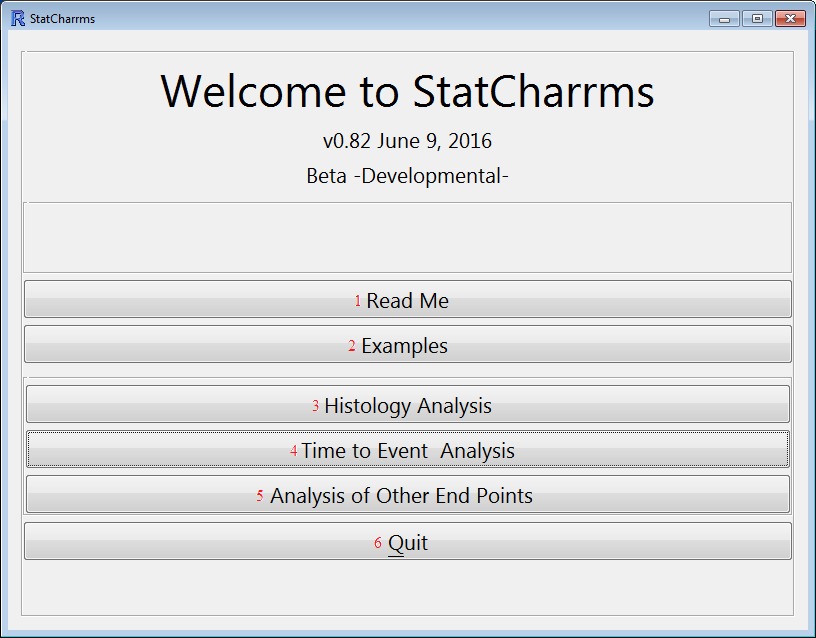
\includegraphics[width=\textwidth,keepaspectratio]{IntroWindow.png}}
\end{center} 

\begin{enumerate}
	
	\item[\begingroup\color{red}1:\endgroup] At the top of the introduction window is the \textbf{[Read Me]} button. 
		The \textbf{[Read Me]} button will display information about the authors, references, and a complete log of developmental changes. 

	\hypertarget{DataExample}{}
	\item[\begingroup\color{red}2:\endgroup] The next button down the list is the \textbf{[Examples]} button. This 
		button will create a folder that is populated with the data and results for 
		every example analysis used in this document. This includes an analysis for fecundity, length, weight,     
		time\textendash{}to\textendash{}effect, and histopathological data. A description of each data file is contained within the documentation 
		for StatCharrms. To view the help files for example data sets type the following into the R console:   
	

\begin{RBox}
> help(eventTimeData)     #For time to event data
> help(fecundityData)     #For fecundity data
> help(lengthWeightData)  #For length and weight data
> help(exampleHistData)   #For histological data
\end{RBox}	
	
	These data sets are used for the examples presented in this document, the '\textbf{eventTimeData}' data set is used in the \hyperlink{Time2Event}{\textbf{[Time to Event Analysis]}},
	the  '\textbf{lengthWeightData}' data set in the \hyperlink{OtherEnd}{\textbf{[Analysis of Other Endpoints]}}, and the '\textbf{eventTimeData}' is used in the examples for
	the \href{https://cran.r-project.org/web/packages/RSCABS/vignettes/RSCABS.pdf}{\textbf{[Histology Analysis]}}.
	
	
	\item[\begingroup\color{red}3:\endgroup] Next is the \hyperlink{Histopath}{\textbf{[Histology Analysis]}}
		button. This button calls Histopath() from the RSCABS package allowing for the analysis of data sets from 
		histopathological endpoints. Since the package RSCABS is a stand alone package called by the 
		\hyperlink{Histopath}{\textbf{[Histology Analysis]}}
		button, directions on the module's use are not stated in this document. 
		Instead directions on how to use the the module can be found  
		\href{https://cran.r-project.org/web/packages/RSCABS/vignettes/RSCABS.pdf}{here on the CRAN website}. 
		

	\item[\begingroup\color{red}4:\endgroup] Continuing down the list is the \hyperlink{Time2Event}{\textbf{[Time to Event Analysis]}} button, which calls the
		window used in performing Cox proportional mixed effect models [\hyperlink{R13}{13}, \hyperlink{R15}{15}].
	
	\item[\begingroup\color{red}5:\endgroup] The \hyperlink{OtherEnd}{\textbf{[Analysis of Other Endpoints]}} 
		button is used for analysis on quantitative endpoints (such as length, weight, and fecundity) using the following statistical tests:   
		ANOVA, repeated measures ANOVA, mixed effects ANOVA, weighted ANOVA, Dunn's test [\hyperlink{R1}{1}], Dunnett's test [\hyperlink{R2}{2}], 
		a step down Jonckheere\textendash{}Terpstra (JT) trend test 
		[\hyperlink{R7}{7},\hyperlink{R10}{10},\hyperlink{R14}{14}], and Williams test [\hyperlink{R2}{2},\hyperlink{R17}{17}].  
	
	
	\item[\begingroup\color{red}6:\endgroup] Last and mostly definitely least is the \textbf{[Quit]} button which closes both StatCharrms and R. 
	
\end{enumerate}	
	



\section*{Histology Analysis}
\label{sec:Histopath}
\thispagestyle{plain}
\addcontentsline{toc}{section}{Histology Analysis}	
\hypertarget{Histopath}{}

			
	StatCharrms uses RSCABS to perform it's histology analysis and since RSCABS is a stand only package and thus the 
	directions on it's use and not repeated in this document.  To find directions on it's use click the 
	\href{https://cran.r-project.org/web/packages/RSCABS/vignettes/RSCABS.pdf}{this link} to the the vignette on the CRAN website 
	or if Run.StatCharrms() has been, called the RSCABS vignette can be opened by typing the following
	into the R Console:		
		
\begin{RBox}
> vignette('RSCABS')	
\end{RBox}	
	
	

  

\hypertarget{Time2Event}{\section*{Time to Event Analysis}}

\label{sec:Time2Event}
\addcontentsline{toc}{section}{Time to Event Analysis}
\subsection*{Time to Event Analysis Main Window}
\label{subsec:Time2EventMain}
\addcontentsline{toc}{subsection}{Time to Event Analysis Main Window}


	Pressing the \textbf{[Time to Event Analysis]} button on the  \hyperlink{fig:IntroWindow}{StatCharrms introductory window} 
	will generate the \textbf{Time to Event Analysis} window. 
	

\begin{center}
\hypertarget{fig:Time2Event2}{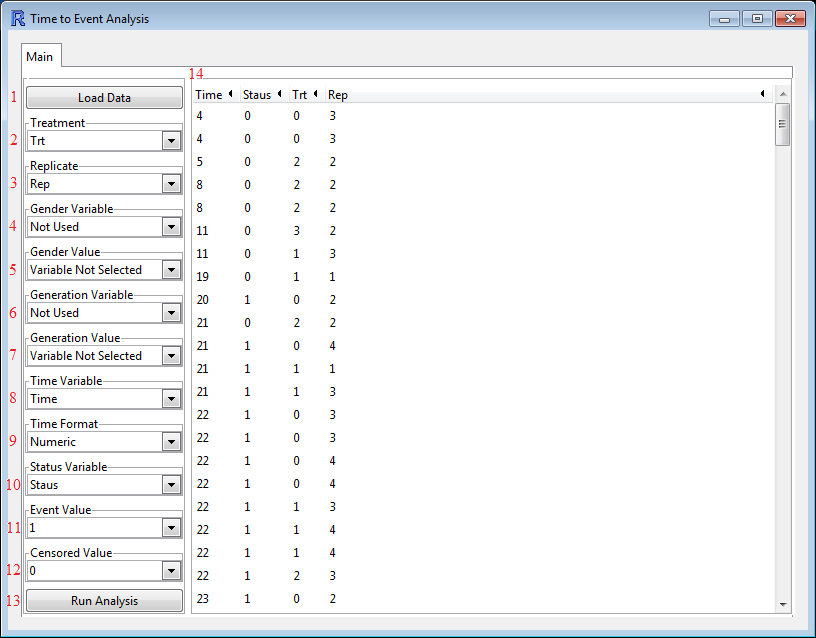
\includegraphics[width=\textwidth,keepaspectratio]{Time2Event2.png}}
\end{center} 

At first only the \textbf{[Load Data]} Button (\textcolor{red}{1}) will be available.  Pressing this button will 
call a dialogue box where a data set can be navigated to and selected. Data files must be in csv format, 
the first row must contain 
the header information, and each additional row contain information about an observation.  After the data is loaded items  
\textcolor{red}{2\textendash{}13} will appear while (\textcolor{red}{14}) will contain the loaded data. Information
about each item in the window is listed below:    
    
\begin{enumerate}

\item[\begingroup\color{red}1:\endgroup] The \textbf{[Load Data]} button is used to load a data set into StatCharrms. 

\item[\begingroup\color{red}2:\endgroup] The name of the \textbf{Treatment} variable, where the lowest number indicates controls and every greater number is a more severe treatment.  
	This must be selected for any analysis to run.
	
\item[\begingroup\color{red}3:\endgroup] The name of the \textbf{Replicate} variable.  The \textbf{Replicate} variable may 
	either contain character strings or numeric values. 

\item[\begingroup\color{red}4:\endgroup] Used to specify the name of the \textbf{Gender Variable}, if applicable.

\item[\begingroup\color{red}5:\endgroup] \textbf{Gender Value}: If a variable for gender is specified, the value of the gender used in the analysis is specified here. 

\item[\begingroup\color{red}6:\endgroup] The \textbf{Generation Variable} is used if the experiment spanned multiple generations. This is where the name of the variable that contains 
	information about each generation can be specified.

\item[\begingroup\color{red}7:\endgroup] \textbf{Generation Value} is the generation the analysis is performed on and is defined here.

\item[\begingroup\color{red}8:\endgroup] The name of the \textbf{Time Variable} is the name of the variable that indicates when events happen. 
	Values in the column can either be dates or integers representing a period of time since the start of the experiment.  
	This must be selected for any analysis to run.  

\item[\begingroup\color{red}9:\endgroup] \textbf{Time Format}: The format the \textbf{Time Variable} is in. It can be any standard 
	format for date or a number, which is indicated by selecting \textbf{Numeric}. Note, by convention StatCharrms will set the 
	earliest date in the analysis to 0. 

\item[\begingroup\color{red}10:\endgroup] The \textbf{Status Variable} is the variable that indicates the final status of the subject, 
	whether it is the event being tested for or a censoring event (see \textcolor{red}{11} and \textcolor{red}{12}).    

\item[\begingroup\color{red}11:\endgroup]  The \textbf{Event Value} is the value representing the event being tested for. 

\item[\begingroup\color{red}12:\endgroup] The \textbf{Censored Value} is used to indicate the value used to represent a censored event . 

\item[\begingroup\color{red}13:\endgroup] The \textbf{[Run Analysis]} Button can be used after each of the entries for \textbf{Treatment}, \textbf{Status Variable}, and 
	\textbf{Event Value} have been specified. 

\item[\begingroup\color{red}14:\endgroup] This is were the data set is displayed.  
	Always double check the data set to make sure it was loaded correctly.  

\end{enumerate}


\label{subsec:Time2EventResults}
\subsection*{Time to Event Results}
\addcontentsline{toc}{subsection}{Time to Event Results}

After all the values have been specified pressing the \textbf{[Run Analysis]} button (\textcolor{red}{13}) will run a 
mixed effects Cox proportional hazards analysis on the data, then generate the \textbf{Time to Event Results} window. 

\begin{center}
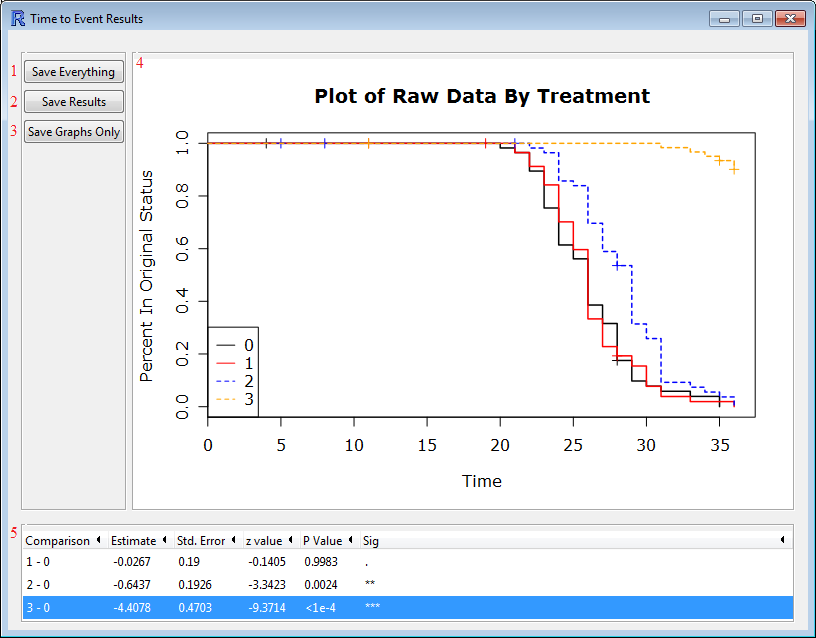
\includegraphics[width=\textwidth,keepaspectratio]{Time2Event3.png}
\end{center} 

\begin{enumerate}

\item[\begingroup\color{red}1:\endgroup] The \textbf{[Save Everything]} button will save the graph being displayed (\textcolor{red}{4})
	as a pdf. Furthermore, this button will also save the main effect table (\textcolor{red}{5}) and the \hyperlink{fig:Time2Event2}{data table} as an HTML file. 

\item[\begingroup\color{red}2:\endgroup] The \textbf{[Save Results]} button will save the 
	\hyperlink{fig:Time2Event2}{data table} and the main effect table (\textcolor{red}{5}) as an HTML file. 

\item[\begingroup\color{red}3:\endgroup] The \textbf{[Save Graphs Only]} button will save the graph being displayed (\textcolor{red}{4})
	as a pdf.
	
\item[\begingroup\color{red}4:\endgroup] A Kaplan\textendash{}Meier plot [\hyperlink{R8}{8}].  This plot does not take into account the replicate structure of the data.  

\item[\begingroup\color{red}5:\endgroup] The main effects table [\hyperlink{R6}{6}].  This table displays the results of a Dunnett's test from the Cox mixed effects models.  The columns are:
	\begin{itemize}
		\item \textbf{Comparison}: The treatment levels being compared.
		\item \textbf{Estimate}: The estimated difference between the treatment and the controls.
		\item \textbf{Std.Error}:  The estimated difference between treatment levels.
		\item \textbf{z value}: The value of a z statistic.
		\item \textbf{P Value}: The corresponding p\textendash{}value of the Dunnett's test.
		\item \textbf{Sig}: A significance flag where ``.'' is a p\textendash{}value > 0.05, ``*'' is
			a 0.01 < p\textendash{}value $\leq$  0.05, ``**'' for 0.001 < p\textendash{}value $\leq$  0.01, and ``***'' for p\textendash{}value $\leq$  0.001.  	
	\end{itemize}

\end{enumerate}

 

\hypertarget{OtherEnd}{\section*{Other Endpoints}}
\label{sec:OtherEnd}
\addcontentsline{toc}{section}{Analysis of Other Endpoints}
\label{subsec:OtherEndpointsMain}
\subsection*{Other Endpoints Main Window}
\addcontentsline{toc}{subsection}{Other Endpoints Main Window}


	This module of StatCharrms  is used for endpoints with standard numerical values. Length, weight, and fecundity 
	are examples of data with standard numerical values.  
	When the \textbf{[Analysis of Other Endpoints]} button is pressed on the 
	\hyperlink{fig:IntroWindow}{StatCharrms introductory window}, the main analysis window for other endpoints 
	will appear. 
	
	
	\begin{center}
	\hypertarget{fig:OEMain}{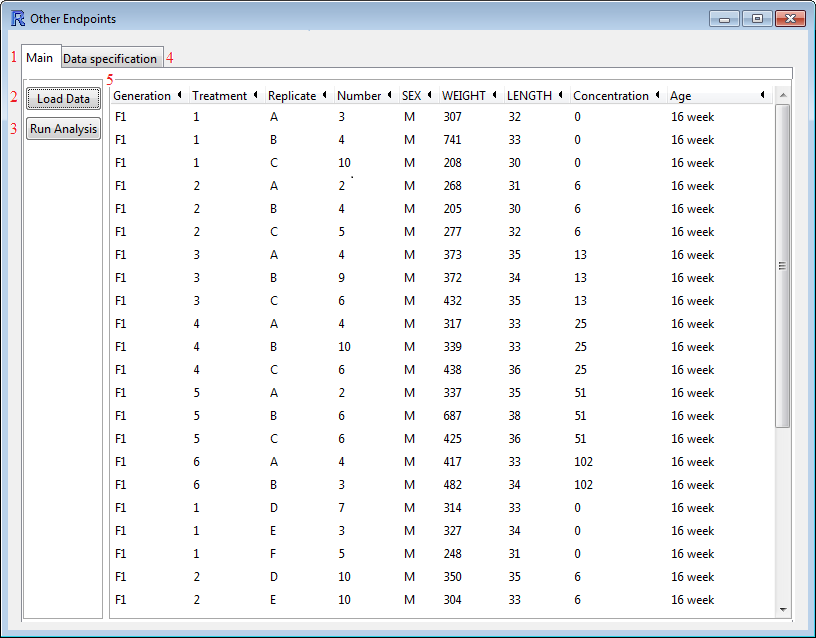
\includegraphics[width=\textwidth,keepaspectratio]{StandardAnl2.png}}
	\end{center} 

	\begin{enumerate}
		\item[\begingroup\color{red}1:\endgroup] The \textbf{Main} tab for the \textbf{Analsis of Other Endpoints}
			module.  Items on this tab are used to load, view, and analyze standard numerical data.
			
		\item[\begingroup\color{red}2:\endgroup] The \textbf{[Load Data]} button is used to load data into 
			StatCharrms. After data is loaded a \textbf{Data specification} tab (\textcolor{red}{4}) will be 
			created and (\textcolor{red}{5}) will be updated with the data set.
			
		\item[\begingroup\color{red}3:\endgroup] The \textbf{[Run Analysis]} button will only appear after the 
			\textbf{[Confirm Selected Values and Variable]} button is pressed on the \hyperlink{fig:DataSpecTab}{\textbf{Data specification}} tab.
			Pressing this button will start running the analyses selected on the \hyperlink{fig:DataSpecTab}{\textbf{Data specification}} tab.
			After every analysis is ran a new window will appear with the results of each analysis.
			
		\item[\begingroup\color{red}4:\endgroup] The \hyperlink{fig:DataSpecTab}{\textbf{Data specification}} tab 
			only appears after a data set has been loaded into StatCharrms.  This tab is where information about 
			the data is specified. If a new specification on the same data set is desired the 
			\hyperlink{fig:DataSpecTab}{\textbf{Data specification}} tab can be navigated back to and changes 
 			can be made.
			After changes are made just press the \textbf{[Confirm Selected Values and Variables]} button on the 
			\hyperlink{fig:DataSpecTab}{\textbf{Data specification}} tab to lock in the changes.  
			
		\item[\begingroup\color{red}5:\endgroup] This is where the current data set is displayed.  If any of the 
			\textbf{generation}, \textbf{gender}, and/or \textbf{age} values (all of which are optional) are selected on the \hyperlink{fig:DataSpecTab}{\textbf{Data specification}} tab,
			the selection will be reflected here by subsetting the data. 
			
	\end{enumerate}	
	
\label{subsec:OtherEndpointsSpec}
\subsection*{Other Endpoints Specification Tab}
\addcontentsline{toc}{subsection}{Other Endpoints Specification Tab}}
	
\hypertarget{fig:DataSpecTab}{} 
\begin{center}
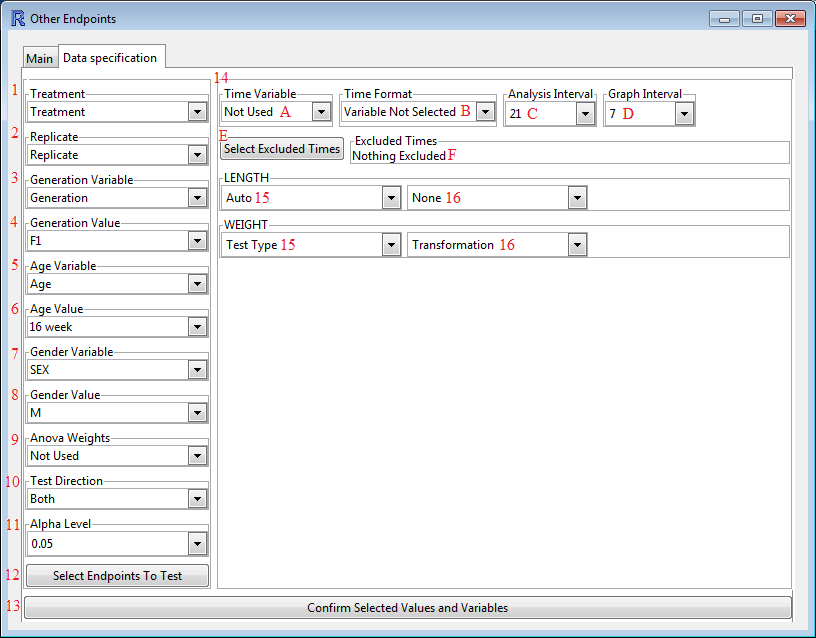
\includegraphics[width=\textwidth,keepaspectratio]{StandardAnl3.png}
\end{center} 


\begin{enumerate}

\item[\begingroup\color{red}1:\endgroup] This is where the name of the \textbf{Treatment} variable is specified. 
	The \textbf{Treatment} variable must contain only numbers where the lowest number indicates controls and 
	every greater number indicates a more severe treatment. Typically this is 1 for controls, 2 for the next highest treatment and so forth.   
	A \textbf{Treatment} variable must be specified before analysis can start. 

	
\item[\begingroup\color{red}2:\endgroup] The name of the \textbf{Replicate} variable. Values for the \textbf{Replicate} variable
	can be any combination of number and letters. 
 
\item[\begingroup\color{red}3:\endgroup] The name of the \textbf{Generation Variable}. Declaring a \textbf{Generation Variable} is optional. 

\item[\begingroup\color{red}4:\endgroup] If different generations are used the \textbf{Generation Value} is the generation the analysis is performed on. 
	
\item[\begingroup\color{red}5:\endgroup] The name of the \textbf{Age Variable}. Declaring a \textbf{Age Variable} is optional.

\item[\begingroup\color{red}6:\endgroup] If there are multiple ages within the data set, the \textbf{Age Value} is the age that the analysis is performed on is
	specified here.

\item[\begingroup\color{red}7:\endgroup] The name of the \textbf{Gender Variable}.  Declaring a \textbf{Gender Variable} is optional.

\item[\begingroup\color{red}8:\endgroup] \textbf{Gender Value}: The gender the analysis is performed on. 

\item[\begingroup\color{red}9:\endgroup] If a weighted ANOVA is to be used, the \textbf{ANOVA Weight} is the name of the variable 
	containing the weights for the ANOVA. 

\item[\begingroup\color{red}10:\endgroup] The \textbf{Test Direction} can be set to \textbf{Both} for a two\textendash{}tailed test or either of; 
	\textbf{Decreasing} or \textbf{Increasing} for a one\textendash{}tailed test.  Since MEOGRT [\hyperlink{R11}{11}] calls for one\textendash{}tailed test, the default	
	setting is \textbf{Decreasing}.

\item[\begingroup\color{red}11:\endgroup] The \textbf{Alpha Level}. This is only used in the 
	\hyperlink{aly:JT}{Jonckheere-Terpstra trend test}.  
    The p\textendash{}value of a step of the  \hyperlink{aly:JT}{Jonckheere-Terpstra trend test} needs to be less then the \textbf{Alpha Level} for the test 
	to proceed to the next step. \textbf{Alpha Level} is also used to set the confidence intervals for the \hyperlink{fig:OEResults}{Summary Table} and the
	\hyperlink{fig:Dunnett}{Dunnett Table}.
 	
\item[\begingroup\color{red}12:\endgroup] After a \textbf{Treatment} variable is specified the 
	\textbf{[Select Endpoints To Test]} button
	can be pressed to specify every endpoint an analysis is performed on. 
	Each selected endpoint will appear in (\textcolor{red}{14}) contained 
	within a frame named after the endpoint.
	
\item[\begingroup\color{red}13:\endgroup] After endpoints are selected the \textbf{[Confirm Selected Values and Variables]} 
	button is used to update StatCharrms with all the values specified in this form.  At any time the 
	\textbf{Data specification} tab can be navigated back to and the values of the entries can be changed. 
	After the changes are made pressing the \textbf{Confirm Selected Values and Variables} button will update the information in StatCharrms.

\item[\begingroup\color{red} 14:\endgroup] At first this will only contain \textcolor{red}{A\textendash{}F}, however after endpoints are specified it will also
	contain a frame for each endpoint selected.

\item[\begingroup\color{red} A\textendash{}F:\endgroup] These selections are only used if repeated observations on the same subject are 
	recorded during different times over the course of the study. These values selected in \textcolor{red}{A\textendash{}F} apply to all endpoints. 
	
	\begin{enumerate}
		\item[\begingroup\color{red}A:\endgroup] The name of the \textbf{Time Variable}, which indicates when the observation occurred.
		
		\item[\begingroup\color{red}B:\endgroup] If the time is listed as dates, the \textbf{Time Format} is used to specify the format the date is in. 
			The \textbf{Time Variable} can also be a list of numbers, in which case (\textcolor{red}{B}) can be set to \textbf{Numeric}.
		
		\item[\begingroup\color{red}C:\endgroup] The \textbf{Analysis Interval} is the number of units in time (e.g. number of days) each endpoint is averaged over for the analysis.  

		\item[\begingroup\color{red}D:\endgroup] The \textbf{Graph Interval} is the number of units in time (e.g. number of days) each endpoint is averaged over for the 
			purpose of graphing.  
		
		\item[\begingroup\color{red}E:\endgroup] The \textbf{[Select Excluded Times]} button allows for the selection of each time to be excluded from the analysis. 
		
		\item[\begingroup\color{red}F:\endgroup] Every excluded time will be displayed within this frame.
		
	\end{enumerate}

\item[\begingroup\color{red} 15\textendash{}16:\endgroup] Appear after endpoints are selected.  Each selected endpoint will generate a frame whose name corresponds to the name of the  endpoint.  
	In the example above the endpoints LENGHT and WEIGHT [sic] were selected from the data set. 
	
	\begin{enumerate}
		\item[\begingroup\color{red}15:\endgroup] \textbf{Test Type} controls for the specific type of statistical test used for that endpoint.  
			This can be set to \textbf{Auto}, which follows \hyperlink{fig:FlowChart}{MEOGRT guidelines}, or any 
			specific test type the StatCharrms is capable of performing.

		\item[\begingroup\color{red}16:\endgroup] The \textbf{Transformation} used on the endpoint. As with (\textcolor{red}{15}) this only appears after an endpoint is selected.  
			This can be \textbf{None} for no transformation, \textbf{Square\_Root} commonly used for count data,
			\textbf{Log}  (base 10) for data that spans multiple orders of magnitude, \textbf{Log + 1} if 
			the data both spans multiple orders of magnitude and includes a value of 0, and finally \textbf{Arcsine} (of the square root of the response)
			for analysis of percents.
			
	\end{enumerate}
\end{enumerate}	
	
	After the \textbf{[Confirm Selected Values and Variables]} button is pressed, the analysis can be ran from the 
	\hyperlink{fig:OEMain}{\textbf{Main}} tab 
	using the \textbf{[Run Analysis button]}. This will start analyzing every endpoint. 
	After every analysis is finished (which may take a while) the results window will appear.  

	
\label{subsec:OtherEndpointsResults}
\subsection*{Other Endpoints Results}
\addcontentsline{toc}{subsection}{Other Endpoints Results}}
	

\begin{center}
\hypertarget{fig:OEResults}{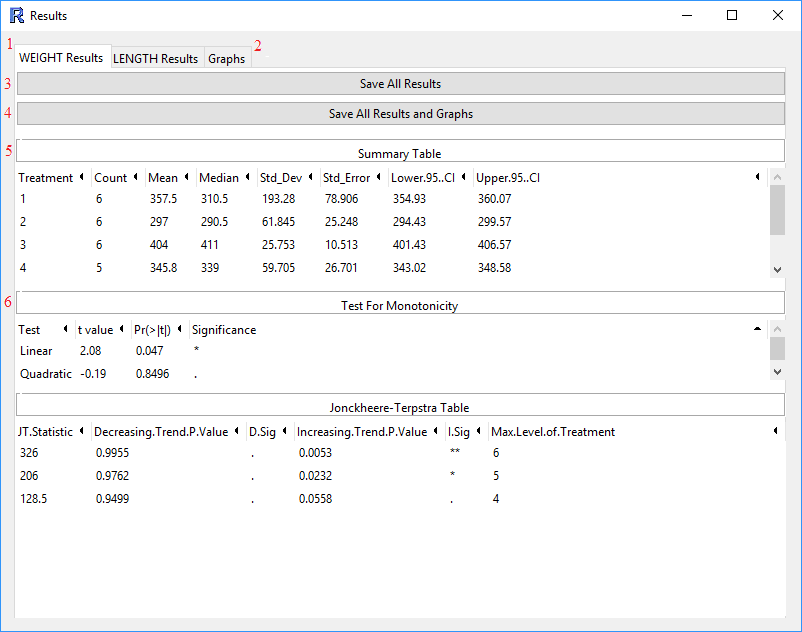
\includegraphics[width=\textwidth,keepaspectratio]{StandardAnl5-New.png}}
\end{center} 


\begin{enumerate}	
	
	\item[\begingroup\color{red}1:\endgroup] The endpoint tabs.  There is a tab for every endpoint used in the analysis.  

	\item[\begingroup\color{red}2:\endgroup] Clicking on the \textbf{Graphs} tab will navigate you to a 
		\hyperlink{Sec:GraphTab}{tab were the data can be plotted}.    
	
	\item[\begingroup\color{red}3:\endgroup] The \textbf{[Save All Results]} button will save all the 
		results (and data tables) for all the endpoints as HTML files.
	
	\item[\begingroup\color{red}4:\endgroup] The \textbf{[Save All Results and Graphs]} button will perform the 
		same operations as the \textbf{[Save All Results]} button with the addition of saving every possible 
		graph for every endpoint as a pdf.  
	
	\item[\begingroup\color{red}5:\endgroup] The \textbf{Summary table} is included in every analysis, and includes entries for:
		\begin{itemize}
			\item \textbf{Treatment}: The level of the treatment variable.
			\item \textbf{Count}: The number of observations for the level of the treatment variable.
			\item \textbf{Mean}:  The mean of the response for the level of the treatment variable.
			\item \textbf{Median}: The median of the response for the level of the treatment variable.
			\item \textbf{Std\_Dev}: The standard deviation of the response for the level of the treatment variable.
			\item \textbf{Std\_Error}: The standard error of the response for the level of the treatment variable.
			\item \textbf{Lower.##..CI}: The lower 1-alpha percent (defaults to 95 percent) confidence interval of the mean value of the response for the treatment level. 
			\item \textbf{Upper.##..CI}: The upper 1-alpha percent (defaults to 95 percent) confidence interval of the mean value of the response for the treatment level. 
		\end{itemize}
		
	\item[\begingroup\color{red}6:\endgroup] The rest of the tables depends on which analyses were ran.  The two tables 
		listed \hyperlink{fig:OEResults}{in the figure above} are the \textbf{Test For Monotonicity} table and 
		the \textbf{Johnckheere\textendash{}Terpstra table}. Other tables could include: a \textbf{Wilks table}, 
		a \textbf{Levene table}, a \textbf{Anova table}, a \textbf{Dunnett table}, and a \textbf{Dunns table}.  
		A description for each table is listed below.
		
		
		
		
		\begin{itemize}
			\item \textbf{Test For Monotonicity}: This is the test for monotonicity as described in the OECD 
				guidance for statistics [\hyperlink{R10}{10}]. According to the test, data is considered to be monotonic unless a \textbf{Quadratic} 
				term is significant and the \textbf{Linear} term is not. 
				The columns of the table are described below:
				
				\hypertarget{fig:MonoTest}{}
				\begin{center}
				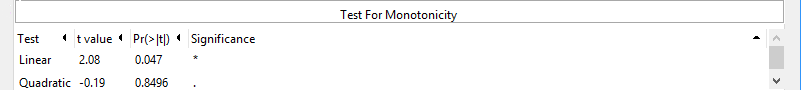
\includegraphics[width=\textwidth,keepaspectratio]{MonoTest-New.png}
				\end{center} 
				
				\begin{itemize}
					\item \textbf{Test}: The test for a linear or quadratic trend. 
					\item \textbf{t value}: The t\textendash{}value for that test.
					\item \textbf{Pr(>|t|)}: The associated p\textendash{}value.
					\item \textbf{Significance}: A significance flag where  ``.'' is a p\textendash{}value > 0.05, ``*'' is
						a 0.01 < p\textendash{}value $\leq$  0.05, ``**'' for 0.001 < p\textendash{}value $\leq$  0.01, and ``***'' for p\textendash{}value $\leq$  0.001.  
				\end{itemize}


			\item \hypertarget{aly:JT}{\textbf{Johnckheere\textendash{}Terpstra table}}: This is the table associated with the step down Johnckheere\textendash{}Terpstra test for trend.	
				This test will keep stepping down until a non\textendash{}significant result is found. 
			
			
				\begin{center}
				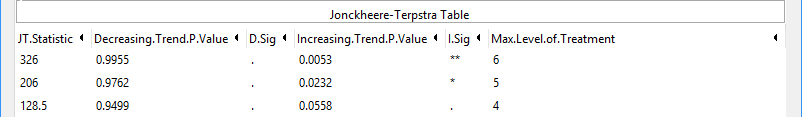
\includegraphics[width=\textwidth,keepaspectratio]{JTTest-New.png}
				\end{center} 
		
				\begin{itemize}
					\item \textbf{JT.Statistic}: The Johnckheere\textendash{}Terpstra test statistic. 
					\item \textbf{Decreasing.Trend.P.Value}: The p\textendash{}value for a decreasing trend.
					\item \textbf{D.Sig}: The significance flag for the decreasing tend where ``.'' is a p\textendash{}value > 0.05, ``*'' is
						a 0.01 < p\textendash{}value $\leq$  0.05, ``**'' for 0.001 < p\textendash{}value $\leq$  0.01, and ``***'' for p\textendash{}value $\leq$  0.001. 
					\item \textbf{Increasing.Trend.P.Value}: The p\textendash{}value for a increasing trend.
					\item \textbf{I.Sig}: The significance flag for the increasing tend where ``.'' is a p\textendash{}value > 0.05, ``*'' is
						a 0.01 < p\textendash{}value $\leq$  0.05, ``**'' for 0.001 < p\textendash{}value $\leq$ 0.01, and ``***'' for p\textendash{}value $\leq$  0.001.
					\item \textbf{Max Level of Treatment}: The treatment level the test statistic corresponds to.	
				\end{itemize}	
			
			
			
			
			\item \textbf{Wilks table}: A table for the Shapiro\textendash{}Wilk test for normality, with additional statistics about the 
				data's statistical distribution. 
			
			\hypertarget{fig:Wilks}{}			
			\begin{center}
			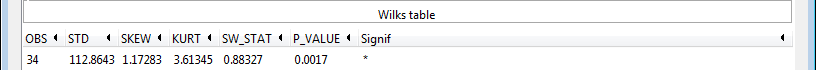
\includegraphics[width=\textwidth,keepaspectratio]{Wilks.png}
			\end{center} 
		
				\begin{itemize}
					\item \textbf{OBS}: The number of observations in the data set. 
					\item \textbf{STD}: The standard deviation of the residuals in the data set. 
					\item \textbf{SKEW}: The skew statistic [\hyperlink{R5}{5}]. Positive skew could indicate the right skewed 
						distribution while a negative skew could indicate the left skewed distribution. 
					\item \textbf{KURT}: The value of the kurtosis of the residuals. Kurtosis [\hyperlink{R16}{16}] is a measure of how heavy tailed a
						distribution is. A large kurtosis could be indicative of an outlier. 
					\item \textbf{SW\_STAT}: The value of the Shapiro\textendash{}Wilk test statistic. 
					\item \textbf{P\_VALUE}: The p\textendash{}value associated with the test statistic. 
					\item \textbf{Signif}: A significance flag which uses ``*'' for p\textendash{}value $\leq$  0.01 and a ``.'' otherwise.
				\end{itemize}	
		

			\item \textbf{Levene table}: The Levene's test is a test for non\textendash{}homogeneity of variance.  
				
				\hypertarget{fig:Leven}{}	
				\begin{center}
				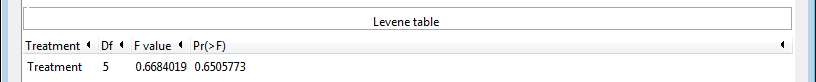
\includegraphics[width=\textwidth,keepaspectratio]{Leven.png}
				\end{center} 
				
				\begin{itemize}
						
					\item \textbf{Df}: The degrees of freedom.  
					\item \textbf{F value}: The value of the test statistic.
					\item \textbf{Pr(>F)}: The p\textendash{}value associated with the test statistic. 
						If the p\textendash{}value is low then the variance 
						is non\textendash{}homogeneous, meaning the Dunnett and ANOVA tests should not be used.  
						In which case either use a different data transformation or use a non-parametric test such as a 
						Johnckheere\textendash{}Terpstra or a Dunns. 
						If the \textbf{Test Type} is set to \textbf{Auto} in the \hyperlink{fig:DataSpecTab}{\textbf{Data specification}} tab, 
						StatCharrms will treat p\textendash{}values less than 0.01 as indicators of non\textendash{}homogeneity. 
				\end{itemize}	
				
	
			
			\item \textbf{Anova table}:
				\hypertarget{fig:Anova}{}	
				\begin{center}
				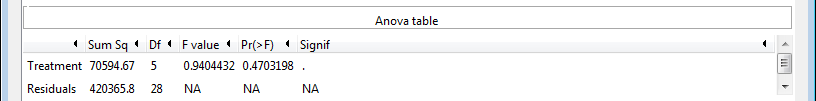
\includegraphics[width=\textwidth,keepaspectratio]{Anova.png}
				\end{center} 
				
				\begin{itemize}
					\item \textbf{Sum Sq}: The between treatment sum of square (top) and the within 
						treatment sum of squares (bottom). 
					\item \textbf{Df}: The degrees of freedom.
					\item \textbf{F value}: The value of the F statistic.
					\item \textbf{Pr(>F)}: The p\textendash{}value associated with the F statistic.
					\item \textbf{Signif}: The significance flag where ``.'' is a p\textendash{}value > 0.05, ``*'' is
						a 0.01 < p\textendash{}value $\leq$  0.05, ``**'' for 0.001 < p\textendash{}value $\leq$  0.01, and ``***'' for p\textendash{}value $\leq$  0.001.
				\end{itemize}	
	
				
		
	
			\item \textbf{Dunnett table}:
			
				\hypertarget{fig:Dunnett}{}	
				\begin{center}
				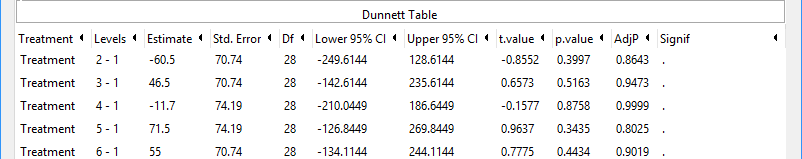
\includegraphics[width=\textwidth,keepaspectratio]{DunnettNew.png}
				\end{center} 
				\begin{itemize}
					\item \textbf{Treatment}: The name of the effect being tested. This is often either the 
						\textbf{Treatment} variable or the \textbf{Time Variable}.
					\item \textbf{Levels}: 	The two levels of effects being tested.  If a \textbf{Time Variable} was not used then
						the comparison will always be with a treatment group to a control. 
					\item \textbf{Estimate}: The estimated difference in transformed means between the levels.  
					\item \textbf{StdErr}: The standard error of the \textbf{estimate}.
					\item \textbf{Df}: The degrees of freedom.  
					\item \textbf{Lower.##..CI}: The lower 1-alpha percent (defaults to 95 percent) confidence interval of the size of the \textbf{Estimate} adjusted for multiple comparisons.
					\item \textbf{Upper.##..CI}: The upper 1-alpha percent (defaults to 95 percent) confidence interval of the size of the \textbf{Estimate} adjusted for multiple comparisons.
					\item \textbf{T.Value}: The values of the student t statistic.
					\item \textbf{P.Value}:	The p\textendash{}value associated with the test statistic.
					\item \textbf{AdjP}:	The p\textendash{}value from the Dunnett's test. 
					\item \textbf{Sig}:	   A significance flag for the p\textendash{}value of the Dunnett's test.  
						An ``.'' is a p\textendash{}value > 0.05, ``*'' is
						a 0.01 < p\textendash{}value $\leq$  0.05, ``**'' for 0.001 < p\textendash{}value $\leq$  0.01, and ``***'' for p\textendash{}value $\leq$  0.001.	
				\end{itemize}	

						
		
		
			\item \textbf{Dunns table}: A non\textendash{}parametric Dunnett's test.  
				This tests for differences in distributions (both mean and variance) in every treatment level
				compared to the controls. 
				
				\hypertarget{fig:Dunns}{}	
				\begin{center}
				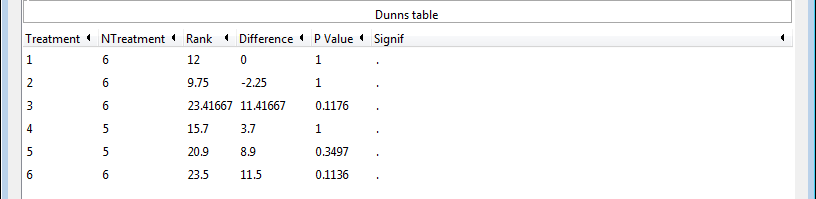
\includegraphics[width=\textwidth,keepaspectratio]{Dunns.png}
				\end{center} 
				\begin{itemize}
				
					\item \textbf{Treatment}: The level of the treatment variable being tested.
					\item \textbf{NTreatment}:  The number of observations for the treatment level.
					\item \textbf{Rank}: The average rank of the data within that treatment.
					\item \textbf{Difference}: The difference in average rank compared to controls.
					\item \textbf{P Value}: The p\textendash{}value associated with the level of treatment.
					\item \textbf{Signif}:	The significance flag where ``.'' is a p\textendash{}value > 0.05, ``*'' is
						a 0.01 < p\textendash{}value $\leq$  0.05, ``**'' for 0.001 < p\textendash{}value $\leq$  0.01, and ``***'' for p\textendash{}value $\leq$  0.001.
						A ``significant'' p\textendash{}value could indicate a difference in either the mean or variance of the data within the treatment 
						compared to the controls. 
			\end{itemize}		
		
		
		
			\item \textbf{Williams Table for Increasing or Decreasing Trend}: This is the Williams test for tend as described in Williams (1973)[\hyperlink{R17}{17}].  This is a parametric test for trend requiring the normality assumption.  
		
				\hypertarget{fig:WillTable}{}	
				\begin{center}
				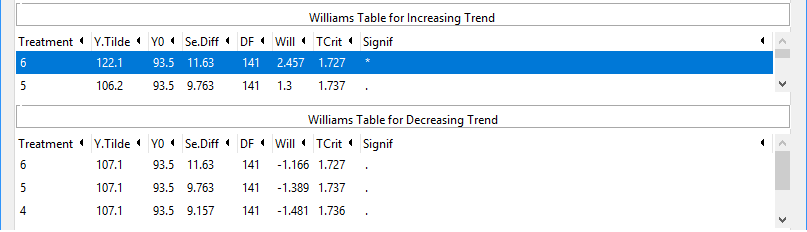
\includegraphics[width=\textwidth,keepaspectratio]{WillTest.png}
				\end{center} 
				\begin{itemize}
					\item \textbf{Treatment}: The level of the treatment variable being tested.
					\item \textbf{Y.Tilde}: This is the amalgamated average [\hyperlink{R3}{3}] for the treatment level.
					\item \textbf{Y0}: The average of the control level.
					\item \textbf{Se.Diff}: The standard error used in the test.
					\item \textbf{DF}: The degrees of freedom.
					\item \textbf{Will}: The test value for the treatment calculated from the Williams test.
					\item \textbf{TCrit}: The critical value for the the Williams test  [\hyperlink{R3}{3}]. This corresponds to to a p\textendash{}value of 0.05.
					\item \textbf{Signif}: A flag indicating the p\textendash{}vlaue.  ``*'' indicates a p\textendash{}value < 0.05 while a ``.'' is a p\textendash{}value $\geq$ 0.05.  
				\end{itemize}
			
		\end{itemize}
\end{enumerate}		


\label{subsec:OtherEndpointsGraphs}
\subsection*{Other Endpoints Graphs}
\addcontentsline{toc}{subsection}{Other Endpoints Graphs}}

Clicking on the \textbf{Graphs} tab will navigate to the graphing portion of the results window. 
Below is an example \textbf{Graphs} tab for the example fecundity data set included in StatCharrms.  	
	
 
	\begin{center}
	\hypertarget{Sec:GraphTab}{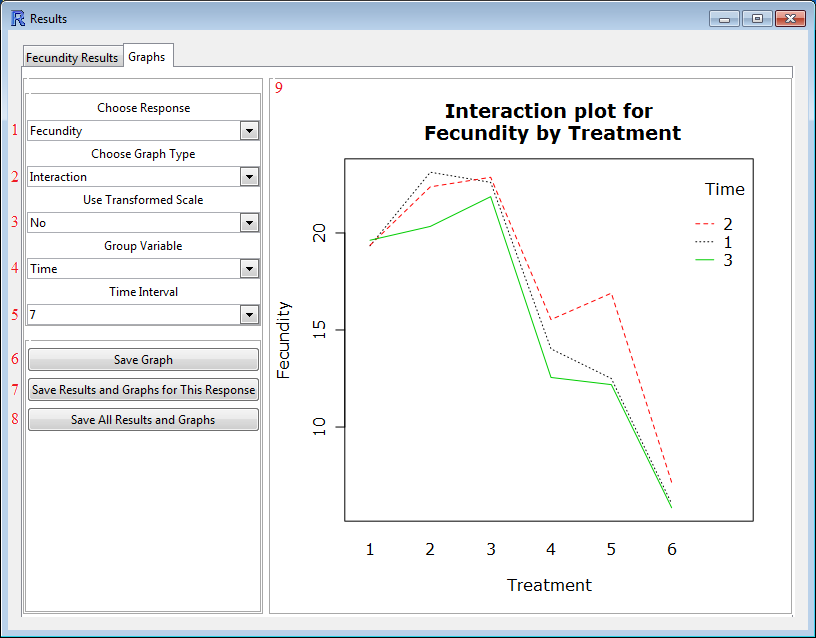
\includegraphics[width=\textwidth,keepaspectratio]{StandardAnl7.png}}
	\end{center} 

	
	\begin{enumerate}
		\item[\begingroup\color{red}1:\endgroup] \textbf{Choose Response} is where the graphed response is chosen. Any endpoint chosen
			on the \hyperlink{fig:DataSpecTab}{\textbf{Data specification tab}} can be selected here. 
			
		\item[\begingroup\color{red}2:\endgroup] \textbf{Choose Graph Type}: This controls the type of graph plotted. Any of a: box and whisker plot, quantile\textendash{}quantile, 
			violin, or (if a \textbf{Time Variable} was specified) an interaction plot can be chosen.   
		
		\item[\begingroup\color{red}3:\endgroup] \textbf{Use Transformed Scale}: This controls the scale the data is plotted in.  Choosing ``No'' plots the data in 
			the untransformed scale, while ``Yes'' will use the transformation selected for the analysis. 
		
		\item[\begingroup\color{red}4:\endgroup] This is only available if a \textbf{Time Variable} was specified
			on the \hyperlink{fig:DataSpecTab}{\textbf{Data specification tab}}.		
			It allows for selection of the variable for the x\textendash{}axis.  This can be either the \textbf{Time Variable}  
			or the  \textbf{Treatment} variable.
		
		\item[\begingroup\color{red}5:\endgroup] This is only available if a \textbf{Time Variable} 
		was specified on the \hyperlink{fig:DataSpecTab}{\textbf{Data specification tab}}.
		 It allows for changing the interval of time the response variable is averaged over. For example, select 1 for a daily response or 7
		 for a weekly one. 
		
		\item[\begingroup\color{red}6:\endgroup] The \textbf{[Save Graph]} button saves the graph currently being displayed as a pdf. 	 
		
		\item[\begingroup\color{red}7:\endgroup] The \textbf{[Save Results and Graph for this Response]} button saves the results for the current response as a HTML file and all possible graphs 
			for the response as a pdf. 
		
		\item[\begingroup\color{red}8:\endgroup] The \textbf{[Save All Results and Graphs]} Saves the results for all responses as a HTML files and all possible graphs 
			for all responses as pdfs. 
		
		\item[\begingroup\color{red}9:\endgroup] A display of the current graph. 			
	\end{enumerate}
	
	
	
\section*{Acknowledgments}
\label{sec:Acknowledgments}
\thispagestyle{plain}
\addcontentsline{toc}{section}{Acknowledgments}	
	I would like to acknowledge Rodney Johnson and Kevin Flynn for their guidance through this project,  Kevin Flynn and Jon Haselman 
	as beta testers,  Tim Dawson as a reviewer of the documentation, and John Green for the source code used in the
	SAS version of StatCharrms. The R version of StatCharrms was built for and paid by the USEPA under Contract 
	EPD\textendash{}13\textendash{}052.
	
		
\section*{References}
\label{sec:References}
\thispagestyle{plain}
\addcontentsline{toc}{section}{References}	

\begin{enumerate}
 \item   \hypertarget{R1}{Dunn, O. J. (1964). Multiple comparisons using rank sums. \textit{Technometrics} \textbf{6}:241\textemdash252.}
	
 \item	 \hypertarget{R2}{Dunnett, C. W. (1955). A multiple comparison procedure for comparing several treatments with a control. 
		\textit{Journal of the American Statistical Association}, \textbf{50}:1096\textendash{}1121.}

 \item	 \hypertarget{R3}{ Green J., Springer T.,  Holbeck H.   \emph{Statistical Analysis of Ecotoxicology Data} (Wiley in press)}
		  

 \item	 \hypertarget{R4}{Green, J. W., Springer, T. A., Saulnier, A. N., and Swintek, J. A. (2014). Statistical analysis of histopathological endpoints. 
		  \textit{Environmental Toxicology and Chemistry}, \textbf{33}(5): 1108\textemdash1116}

\item	 \hypertarget{R5}{Groeneveld, R. and Meeden, G. (1984). Measuring Skewness and Kurtosis. 
		\textit{Journal of the Royal Statistical Society. Series D (The Statistician)} \textbf{33}(4): 391\textemdash399.} 

 \item	 \hypertarget{R6}{Hosmer, D.W. Jr and Lemeshow, S. (1999). \textit{Applied Survival Analysis: Regression Modeling of Time to Event Data}. Wiley\textemdashInterscience. }		
	
 \item	 \hypertarget{R7}{Jonckheere, A. R. (1954). A distribution\textendash{}free k\textendash{}sample test against ordered alternatives.\\ \textit{Biometrika} \textbf{41}:133\textemdash145. }

 \item	 \hypertarget{R8}{Kaplan E. L. and Meier P. (1958). Non\textendash{}parametric estimation from incomplete observations. 
	\textit{Journal of the American Statistical Association } \textbf{53}:457\textemdash481}

 
 \item  \hypertarget{R9}{Lee, E.T. and Wang, J.W., (2003). \textit{Statistical Methods for Survival Data Analysis, 3th edition}.} 
	Wiley\textemdashInterscience. 

 \item  \hypertarget{R10}{OECD, (2014). Current Approaches in the Statistical Analysis of Ecotoxicity Data, OECD	
	Publishing, Paris. \\
	DOI: http://dx.doi.org/10.1787/9789264085275\textemdash{}en }
 
 \item  \hypertarget{R11}{OECD, (2015). Test No. 240: Medaka Extended One Generation Reproduction Test (MEOGRT). OECD	
	Publishing, Paris. \\  DOI: http://dx.doi.org/10.1787/9789264242258\textemdash{}en }
	
 \item  \hypertarget{R12}{OECD, (2015). OECD Guidelines for the Testing of Chemicals, Section 2. Test No. 241: The Larval Amphibian Growth and Development Assay 
	(LAGDA). OECD Publishing, Paris. DOI: http://dx.doi.org/10.1787/9789264242340\textemdash{}en}
 
 \item  \hypertarget{R13}{Ripatti and  Palmgren, J. (2000). Estimation of multivariate frailty models using penalized partial likelihood, \textit{Biometrics} \textbf{56}:1016\textemdash1022. }
 
 \item  \hypertarget{R14}{Terpstra, T. J. (1952). The asymptotic normality and consistency of Kendall's test against trend, when ties are present in one ranking. \textit{Indagationes Mathematicae} \bold{14}:327\textemdash333.}	

 \item  \hypertarget{R15}{Therneau T., Grambsch P., and  Pankratz VS. (2003). Penalized survival models and frailty, \textit{Journal of Computational and Graphical Statistics} \textbf{12}:156\textemdash175. }

 \item  \hypertarget{R16}{Westfall P.H. (2014). Kurtosis as Peakedness, 1905\textendash{}2014. R.I.P.. \textit{The American Statistician} \textbf{68}(3):191\textemdash195, DOI: 10.1080/00031305.2014.917055}

 \item  \hypertarget{R17}{Williams D.A. (1971).  A test for differences between treatment means when several dose levels are compared with a zero dose control. \emph{Biometrics} \bold{27}(1):103\textemdash117. }
 

 
 \end{enumerate}
 


\section*{Appendix}
\label{sec:Appendix}
\thispagestyle{plain}
\addcontentsline{toc}{section}{Appendix}

\label{subsec:FlowChart}
\subsection*{Analysis Flow Chart}
\addcontentsline{toc}{subsection}{Analysis Flow Chart}}	
\hypertarget{fig:FlowChart}{} 


 Flow chart for analysis of other endpoints (Abridged from [\hyperlink{R11}{11}]): 

	\begin{center}
	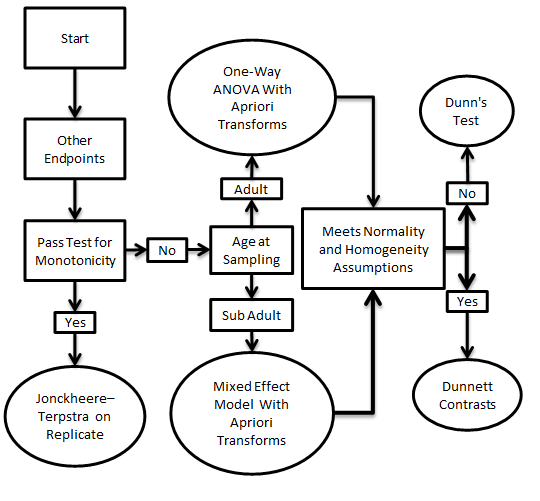
\includegraphics[width=\textwidth,keepaspectratio]{FlowChart.png}
	\end{center} 

	
\label{subsec:RGtk2W}
\subsection*{RGtk2 Version Warning}
\addcontentsline{toc}{subsection}{RGtk2 Version Warning}}	
\hypertarget{fig:RGtk2W}{} 

At the time of writing this, the current version of RGtk2 (2.20.33) does not work with the GUI functions of StatCharrms. 
Trying to use StatCharrms with RGtk2 version 2.20.33 will produce the message below.

  
	\begin{center}
	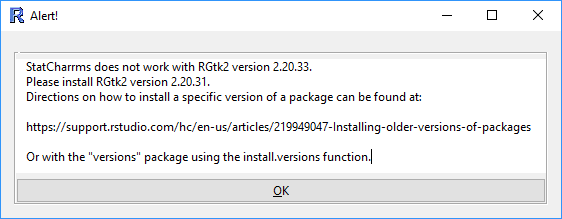
\includegraphics[width=\textwidth,keepaspectratio]{RGtk2W.png}
	\end{center} 

The use the GUI functions of StatCharrms you will need to have the previous version of RGtk2 (2.20.31) installed on your computer. Directions on how to do that can be found \href{https://support.rstudio.com/hc/en-us/articles/219949047-Installing-older-versions-of-packages}{\textbf{[here]}}. If you are using RStudio you could also follow the steps below. 

\begin{enumerate}

	\item Run remove.packages("RGtk2") in the R Console
	\item Download RGtk2 version 2.20.31 as windows binaries from \href{https://cran.r-project.org/web/packages/RGtk2/index.html}{\textbf{the CRAN repository here}}.
	\item	In RStudio, Tools menu Install packages... $\rightarrow$ Install from: Package archive file (.zip; .tar.gz)  $\rightarrow$ select location of RGtk2 $\textunderscore$2.20.31.zip file  $\rightarrow$ install.
	\item	Run library(RGtk) in the R Console for the GTK+ prompt.
	\item	Do you want to install GTK+  $\rightarrow$ yes.
	\item	Restart R.

StatCharrms should now work normally. 
	
	
\end{enumerate}




\end{document}













